\documentclass[12pt, a4paper]{article}
\usepackage[utf8]{inputenc}
\usepackage{amssymb}
\usepackage{indentfirst}
\usepackage{listings}
\usepackage{enumitem}
\usepackage{comment}
\usepackage{graphicx}
\usepackage{color}
\usepackage[portuguese]{babel}
\usepackage{geometry}
\geometry{legalpaper, a4paper,
 total={170mm,257mm},
 left=20mm,
 top=20mm}
\setlength{\voffset}{-10mm}
\definecolor{dkgreen}{rgb}{0,0.6,0}
\definecolor{gray}{rgb}{0.5,0.5,0.5}
\definecolor{mauve}{rgb}{0.58,0,0.82}

\lstset{frame=tb,
  language=Java,
  aboveskip=3mm,
  belowskip=3mm,
  showstringspaces=false,
  columns=flexible,
  basicstyle={\small\ttfamily},
  numbers=none,
  numberstyle=\tiny\color{gray},
  keywordstyle=\color{blue},
  commentstyle=\color{dkgreen},
  stringstyle=\color{mauve},
  breaklines=true,
  breakatwhitespace=true,
  tabsize=3
}

\newcommand{\tit}[1]{\textit{#1}}
\newcommand{\tb}[1]{\textbf{#1}}
\newcommand{\tbi}[1]{\textbf{\textit{#1}}}

\newcommand{\bitem}[2]{ \tb{(\tit{#1}) {#2}}}
\newcommand{\iitem}[1]{(\tit{#1})}

\newcommand{\oo}{orientação à objetos}
\newcommand{\sw}{\tit{software}}
\newcommand{\ssw}{\tit{software} }

\newcommand{\question}[1]{\item \tb{#1}}
\newcommand{\answer}[1]{\par \tb{Resposta:} #1}

\newcommand{\quotes}[1]{``#1''}

\title{Módulo 5 - Atividade Individual \\
  \large Projeto Arquitetural}

\author{Wellington M. Espindula}
\date{Abril de 2021}

\begin{document}
    \maketitle
    
    \begin{enumerate}[label=\textbf{\arabic*.}]
        % Question 1
        \question{Resumo sobre Arquitetura de Software. Com base no podcast que você ouviu, escreva cerca de meia página resumindo o que você aprendeu sobre arquitetura de software, cobrindo ao menos:
            \normalfont{ 
                \begin{enumerate}[label={\alph*.}]
                    \item O que é arquitetura de software;
                    \item Importância da arquitetura de software;
                    \item Decisões relacionadas com a arquitetura de software; e
                    \item Como representar uma arquitetura de software.
                \end{enumerate}}
        }
        \answer{
           Embora existam diversas definições e não uma única consensual, a arquitetura de software rege sobre a estruturação, relacionamento, organização de componentes de um sistema. Segundo Eoin Woods, a Arquitetura de Software é o conjunto de decisões que se tomadas inadequadamente podem causar o cancelamento de um projeto. A partir desta definição, pode-se notar que \tb{a forma como a arquitetura de um sistema é constituída - desde sua concepção até sua evolução - tem o poder de prolongar ou comprometer o ciclo de vida} deste. \\
           Para fins de comparação, podemos imaginar um software \tit{A} sem refatoração constante, repleto de classes deusas altamente acopladas e um software \tit{B} constantemente refatorado para manter módulos com responsabilidades bem definidas e pouco depende entre si. Para modificar o software A, adicionando uma nova regra de negócio, o(s) desenvolver(es) do software A terão dificuldades maiores para fazê-la do que o(s) de B; dado que, em A, haverá de procurar-se por todas as implicações da modificação em diversos trechos de códigos, podendo resultar em novos \tit{bugs} e em novos emaranhados de código; ao passo que, em B, por tentar manter uma \tb{Arquitetura limpa}, a modificação deverá ser realizada em apenas em trechos específicos de código resultando em pouca (ou nenhuma) implicação fora do componente. \\
           Assim percebe-se que \tb{prezar por manter uma arquitetura limpa no processo de planejamento e desenvolvimento de software resulta em maior manutenibilidade} - e até em maior robustez. Portanto, a fim de obter-se uma Arquitetura Limpa em um processo de desenvolvimento, os desenvolvedores deverão sempre realizar decisões acerca de \bitem{i}{Modularização} - A arquitetura deve visar módulos com baixo acoplamento e alta coesão; \bitem{ii}{Separação de Interesses} - Cada módulo deverá ter uma única responsabilidade; \bitem{iii}{Tecnologias} - \tit{Frameworks}, bibliotecas e afins; \bitem{iv}{Requisitos Não-Funcionais} - Requisitos como perfomance, segurança, etc. \\
           Por fim, a fim de representarmos a arquitetura de um software pode-se utilizar desde uma \tb{notação informal} - tomando um módulo como um quadrado, às vezes organizando-os de forma hierárquica ou às vezes usando setas representando dependências, etc -, mas também pode vir a se utilizar \tb{diagramas de pacotes e diagramas de componentes} da UML bem como \tb{ADLs} (Linguagens de Descrição de Arquitetura).
        } \newpage
        
        % Question 2
        \question{Arquitetura de Sistema de Videoconferência. Faça um diagrama da arquitetura de um sistema controlado por computador para vídeo conferência que permite vídeo, áudio, e dados do computador visíveis para vários participantes ao mesmo tempo. O ponto de partida é entender os concerns (preocupações do sistema) e depois estrutura-los, definindo suas dependências.}
        \answer{
           \begin{figure}[!ht]
               \centering
               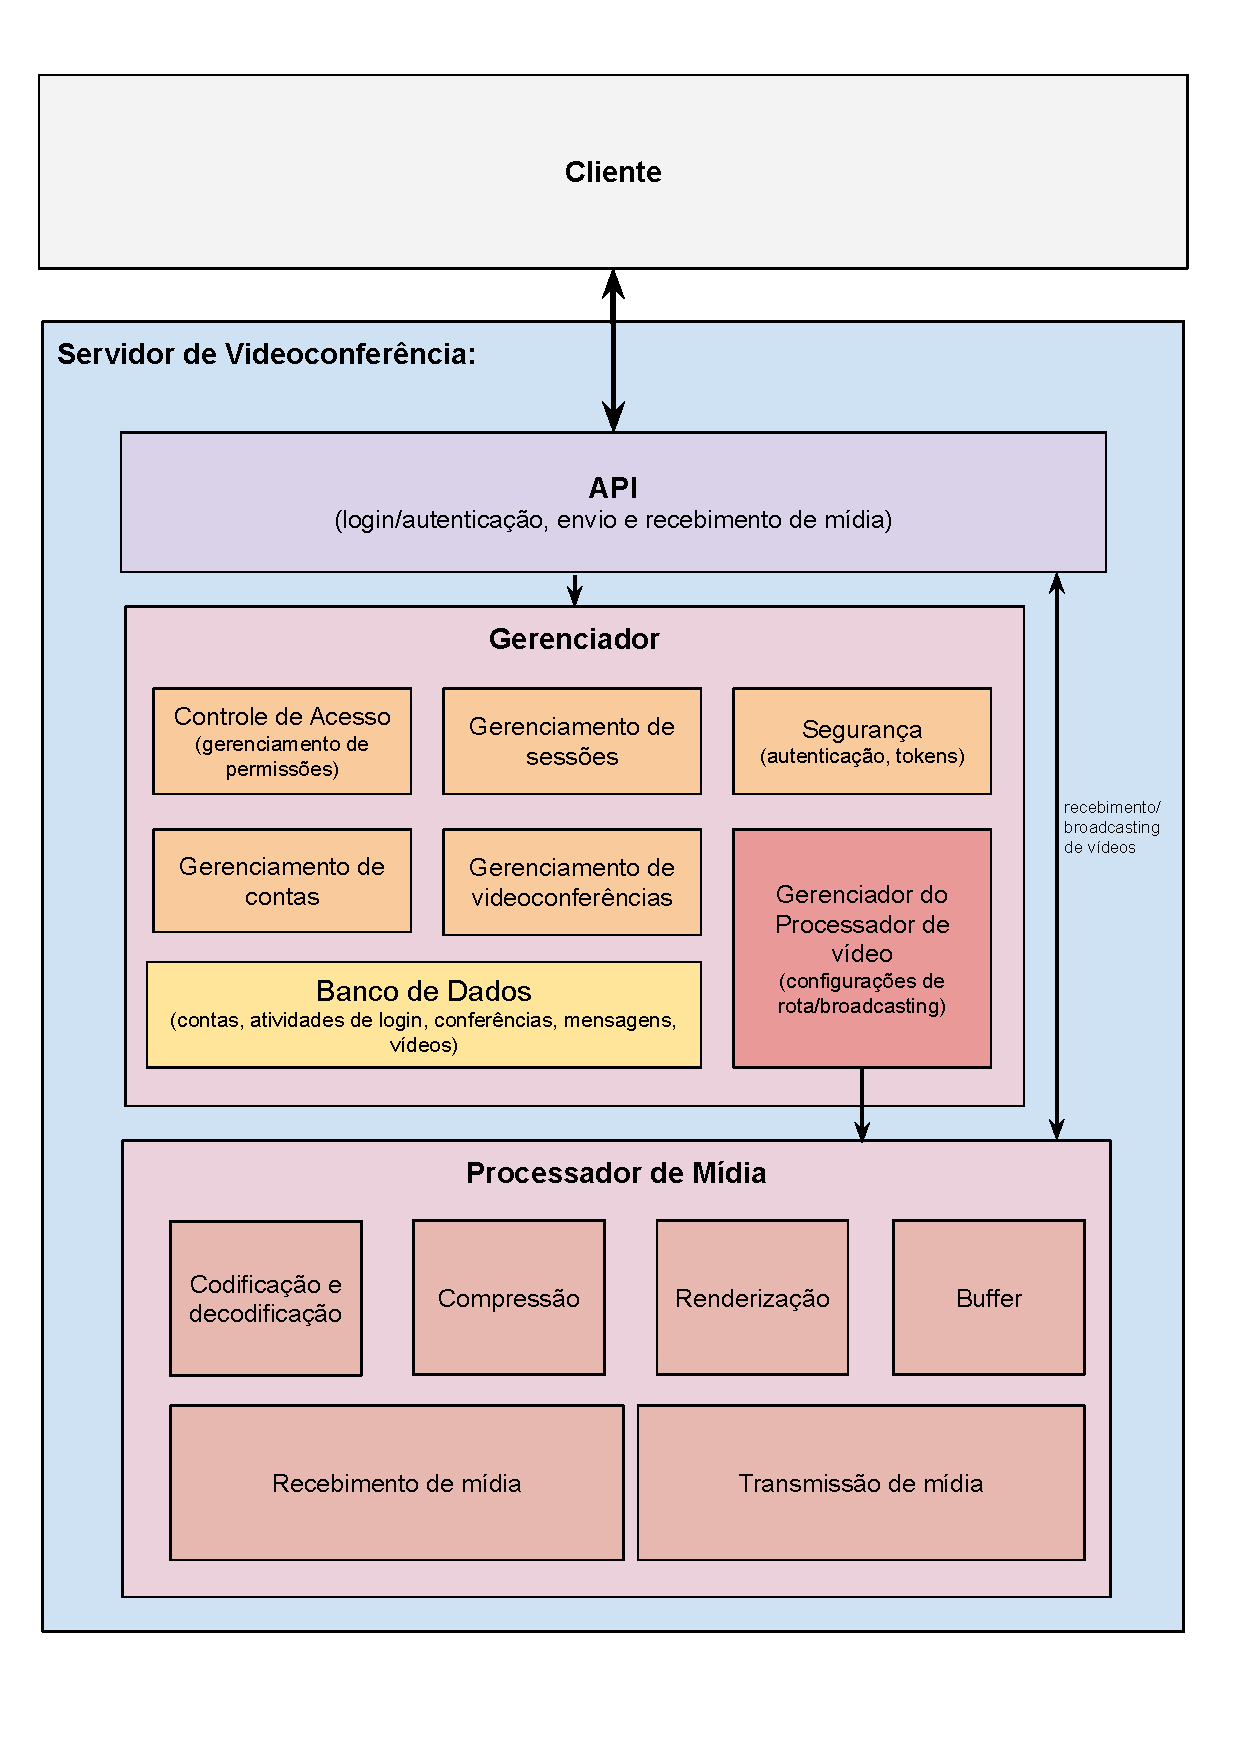
\includegraphics[height=0.8\textheight]{q2.pdf}
                \caption{Diagrama de Arquitetura do Sistema de Videoconferência. Fonte: O Autor, 2021.}
               \label{fig:question2}
           \end{figure}
        } \newpage
        
        % Question 3
        \question{
            Sistema de Biblioteca. Considere o enunciado do sistema de Biblioteca fornecido no módulo anterior e as atividades realizadas anteriormente e faça o seu projeto arquitetura, representando-o através de um diagrama de pacotes.
        }
        \answer{
                \begin{figure}[!ht]
               \centering
               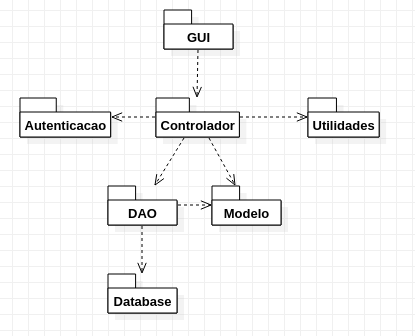
\includegraphics[width=0.85\textwidth]{q3.png}
                \caption{Diagrama de Pacotes do Sistema Biblioteca. Fonte: O Autor, 2021.}
               \label{fig:question2}
           \end{figure}
        }
        \newpage
        
        % Question 4
        \question{Outros Estilos Arquiteturais. Escolha um dos padrões arquiteturais apresentados no PDF “Modulo 5 -Arquitetura de Software - Estilos Arquiteturais Adicionais”, e escreva um parágrafo resumindo o padrão, destacando sua motivação, problema, solução e consequências. Para fazer isso, busque por detalhes sobre o padrão nos PDFs “Modulo 5 - Leitura - [Chapter] Buschmann - Pattern-oriented software architecture (A System of Pattern)” e “Modulo 5 - Leitura -[Chapter] Sommerville - Software Engineering”, e outros identifiquem.}
        \answer{ 
            A arquitetura \tb{Pipe and Filter} surgiu do sistema Unix e se baseia em processos de transformações de entrada de dados gerando saídas. Tais processos podem ser combinados através um \quotes{Pipe} gerando um fluxo de dados entre processos adequados às necessidades. A motivação de usá-la é em sistemas cujos entradas são processadas em diferentes estágio, isto é, uma arquitetura comum para sistemas de processamento de dados. Uma grande vantagem de usar Pipe and filter é que seu estilo é fácil de entender, facilita o reuso e pode ser utilizado em diversos processos de negócios. Um problema é que sua aplicação restringe-se à sistemas textuais; deste modo, é uma solução pouco escalável para sistemas gráficos. Ademais, para que dois processos se comuniquem, eles não podem discordar em termos de estruturas de dados, o que pode ser resolvido forçando concordância de estruturas de dados entre os processos ou mesmo utilizando um processo intermediário de conversão entre duas estruturas de dados.
        }
    
    \end{enumerate}
        
    
\end{document}